\documentclass[12pt, oneside]{report}\usepackage[]{graphicx}\usepackage[]{color}
% maxwidth is the original width if it is less than linewidth
% otherwise use linewidth (to make sure the graphics do not exceed the margin)
\makeatletter
\def\maxwidth{ %
  \ifdim\Gin@nat@width>\linewidth
    \linewidth
  \else
    \Gin@nat@width
  \fi
}
\makeatother

\usepackage{Sweavel}


\usepackage[margin=0.85in]{geometry}
\linespread{1}
\usepackage{xcolor}
\usepackage[colorlinks=false, linkbordercolor=white, citebordercolor=white, 
    filebordercolor=white, urlbordercolor=white]{hyperref}
    
\usepackage{graphicx}
\usepackage[utf8]{inputenc}
\usepackage[english]{babel}
\usepackage[T1]{fontenc}

\usepackage{fancyhdr}
\pagestyle{fancy}
\renewcommand{\headrulewidth}{0.4pt}
\fancyhead{}
\fancyhead[L]{Statictics for Computer Science -- assignment 2} %%% change to your course name and change the number accordingly
\fancyhead[R]{Kanitha Chim} %%% change to your first name and surname
\fancyfoot{}
\fancyfoot[C]{\thepage}

\usepackage{titlesec}
\titlespacing{\chapter}{0pt}{*4}{*2.5}

\titleformat{\chapter}{\normalfont\huge\bf}{\thechapter}{20pt}{\huge\bf}


% Setting up of environment
\usepackage{listings}
\definecolor{dgray}{gray}{0.35} % colour of comments
\definecolor{lgray}{gray}{0.95} % background colour of R-code
\definecolor{llgray}{gray}{0.98} % background colour of R-outputs

\lstdefinestyle{Rstyle}{ % settings of R-code style
language=R, % setting language R
basicstyle=\ttfamily\small, % font and size of R-code
backgroundcolor=\color{lgray}, % background colour of R-code
commentstyle=\ttfamily\small\itshape\color{dgray}, % colour of R comments
showstringspaces=false, % forbidding the highlighting of spaces
numbers=left, % numbering on the left
numberstyle=\ttfamily\small, % font and size of numbering
stepnumber=1, % numbering with step 1
firstnumber=last, % cumulative numbering of rows in consecutive Chunks
breaklines=T} % automatic line breaks of code at the end of a line

\lstdefinestyle{Routstyle}{ %  settings of R-output style
language=R, % setting language R
basicstyle=\ttfamily\small, % font and size of R-output
backgroundcolor=\color{llgray}, % background colour of R-code
showstringspaces=false, % forbidding the highlighting of spaces
numbers=right, % numbering on the right
numberstyle=\ttfamily\small, % font and size of numbering
firstnumber=last, % cumulative numbering of rows in consecutive Chunks
breaklines=T} % automatic line breaks of code at the end of a line

\begin{document}



\begin{titlepage}
    \begin{center}
        \vspace*{1cm}
        
        \Huge
          \textbf{Statistics for Computer Science} %%% change to your course name
        
        \vspace{0.5cm}
        \LARGE
        Assignment 2 %%% change the number accordingly
        
        \vspace{1.5cm}
        
        \textbf{Kanitha Chim} %%% change to your first name and surname
   		  \vspace{1.5cm}
        
        \textbf{501453} %%% change to your UCO
       
        \vfill
        
        Field of Study Software System and Service Management %%% change to your field of study
        
        \vspace{0.8cm}
          \Large
        Faculty of Informatics\\
        Masaryk University\\
        \vspace{0.5cm}
       \today
        
    \end{center}
\end{titlepage}

\addtocontents{toc}{~\hfill\textbf{Page}\par}

\section*{Exercise 3}
\noindent 1. Write down the formula for likelihood function of Poisson distribution.\newline

The formula for the Poisson probability mass function is: \newline

$P(x, \lambda) = \frac{e^{-\lambda} \lambda^{x}}{x!}$ \newline

In Poisson distribution, the parameter of interest is $\lambda$. Having sequence of $X_n$, the probability of observing the sequence $X_n$ will be the product of probabilities of each of them. \newline

Therefore, the kernel of likelihood function of Poisson distribution is: \newline

$L(\lambda|X) = \displaystyle\prod_{i=1}^{N} \frac{\lambda^{X_i} e^{-\lambda}}{X_i !}$ \newline


\noindent 2. Write down the formula for log-likelihood function of Poisson distribution. \newline

The formula for log-likelihood function of Poisson distribution is obtained by using natural logarithm on the likelihood function of Poisson distribution. \newline

Therefore, the kernel of log-likelihood function of Poisson distribution is: \newline

$l(\lambda|X) = ln \left( \displaystyle\prod_{i=1}^{N} \frac{\lambda^{X_i} e^{-\lambda}}{X_i !} \right)$ \newline

$l(\lambda|X) = \displaystyle\sum_{i=1}^{N} X_i ln \lambda - N \lambda$ \newline

\noindent 3. Write down the likelihood equation and work out the exact formula for $\hat{\lambda}$. \newline

$L(\lambda) =  \displaystyle\prod_{i=1}^{N} \frac{e^{-\lambda}\lambda^{x_i}}{x_i !} = e^{-N\lambda} \frac{\lambda^{\sum_{1}^{N}x_i}}{\prod_{i=1}^{N} x_i}$ \newline

$ln L(\lambda) = -N\lambda + \displaystyle\sum_{1}^{N}x_iln(\lambda) - ln\left(\displaystyle\prod_{i=1}^{N} x_i\right)$ \newline

$\frac{dlnL(\lambda)}{dp} = -N + \displaystyle\sum_{1}^{N} x_i \frac{1}{\lambda}$ \newline

$\hat{\lambda} = \frac{\sum_{i=1}^{N}x_i}{N}$ \newline

\noindent 4. Create your own R-function for calculating the value of log-likelihood function of Poisson distribution.
\begin{Schunk}
\begin{Sinput}
x <-c(117, 109, 109, 89, 120, 88, 99, 103, 109, 91, 107, 101, 109, 117, 96, 95, 129, 96, 105, 98)
n <- 20

#the function will take 3 parameters lambda, n and x
#n is number of obervations
#lambda is mean
#x is the sequence of observed values
#finally it will return the value of log-likelihood of Poisson distribution
poi.log.likelihood <- function(lambda, n, x){
  log.like <- sum(x) * log(lambda) - n * lambda
  return(-log.like)
}

ans.poi.log.like <- poi.log.likelihood(mean(x), n, x)
\end{Sinput}
\end{Schunk}
The value of log-likelihood function of Poisson distribution is -7612.856. \newline

\noindent 5. Using function optimize() find $\hat{\lambda}$. Compare it to the estimate you get from the exact formula.
\begin{Schunk}
\begin{Sinput}
#this function will take 2 parameters x and n
#x is the sequence of observed values
#n is number of obervation
#finally it will return lambda hat which is the mean
lambda.hat <- function(x, n){
  return(sum(x)/n)
}
ans.lambda.hat <- lambda.hat(x, n)

#using optimize function to obtain lambda hat
#the optimize function take the log-likelihood of Poisson distribution to optimize with the given interval
#optimize function will return maximum and objective value
#in this case we interest in the value of maximum
lambda.hat.est <- optimize(f = poi.log.likelihood, interval = c(88, 129), maximum = T, x = x, n=n)$maximum
\end{Sinput}
\end{Schunk}
The exact value of $\hat{\lambda}$ is 104.35 and the estimate value of $\hat{\lambda}$ is 128.9999. \newline

\noindent 6. Plot the log-likelihood function, highlight the maximum and denote the maximum likelihood
estimate in plot margin.
\begin{Schunk}
\begin{Sinput}
lambda.hat.seq <- seq(from=88, to=129, length=20)
l.lambda <- apply(X = as.matrix(lambda.hat.seq), MARGIN = 1, FUN = poi.log.likelihood, lambda=ans.lambda.hat, n=n)

plot(lambda.hat.est, ans.poi.log.like, type = 'l', main="log-likelihood function of Poisson Distribution", xlab = bquote(hat(lambda)), ylab = "log-likelihood")
abline(v = lambda.hat.est, col = 'red', lty =2)
abline(h = ans.poi.log.like, col = 'blue', lty = 2)
mtext(bquote(hat(lambda) == .(round(lambda.hat.est, 2))), side = 1, line = 2,
      at = lambda.hat.est, cex = 0.7, col = 'red')
mtext(bquote(log-likelihood == .(round(ans.poi.log.like, 2))), side = 2, line = 2,
      at = ans.poi.log.like, cex = 0.7, col = 'blue')
\end{Sinput}

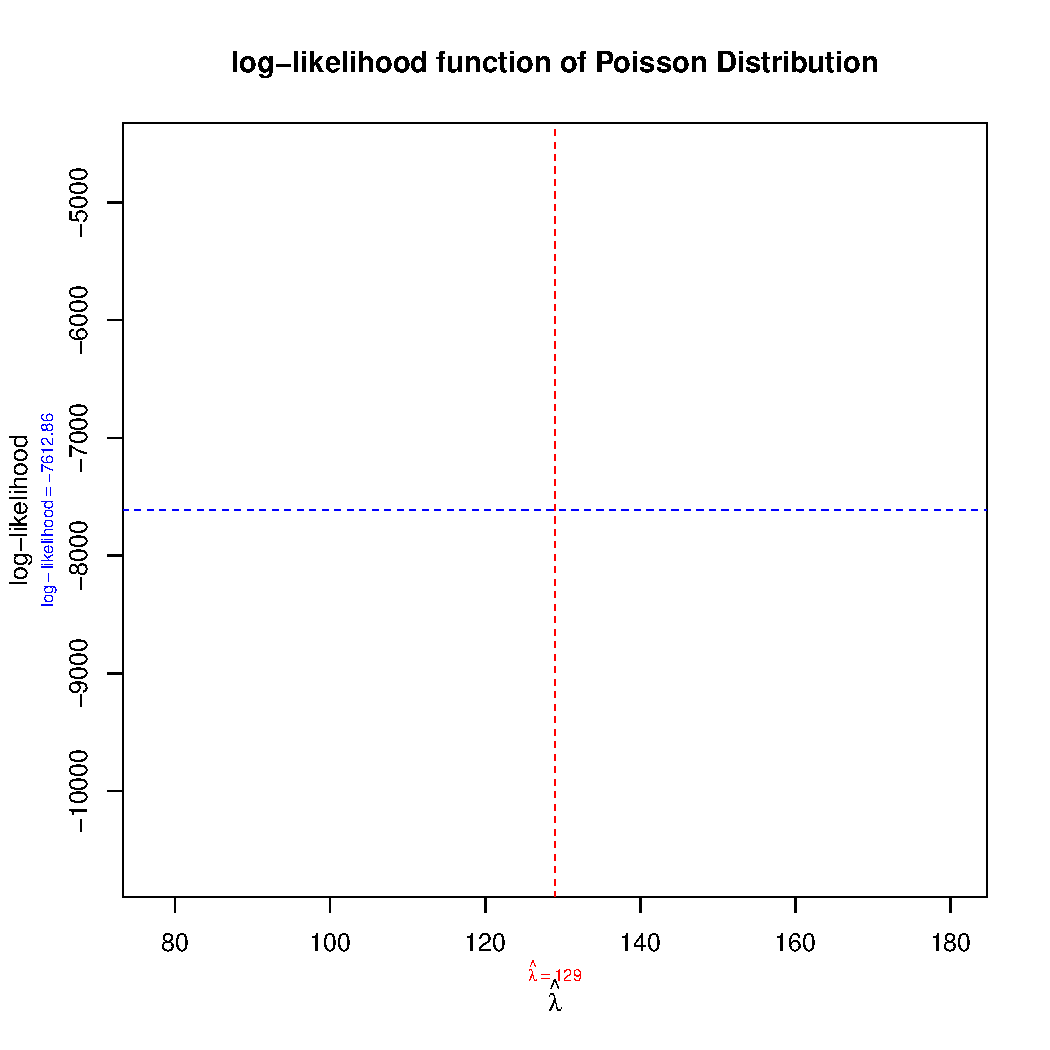
\includegraphics[width=\maxwidth]{figure/unnamed-chunk-3-1} \end{Schunk}

\section*{Exercise 4}
\noindent 1. Write down the null and the alternative hypotheses in mathematical form. \newline

Null hypothesis— $H_0 : \rho = 0$ \newline

Alternative hypothesis— $H_1 : \rho \neq 0$ \newline

\noindent2. Calculate the value of test statistic. \newline
\begin{Schunk}
\begin{Sinput}
setwd(getwd())
body <- read.table(file = 'body-measurements.txt', header = T)
body <- na.omit(body)

body.f.height <- body[body$sex == 'f', 'body.H']
body.f.neck <- body[body$sex == 'f', 'neck.C']

n.x <- length(body.f.height)
n.y <- length(body.f.neck)
mu.x <- mean(body.f.height)
mu.y <- mean(body.f.neck)
sigma2.x <- sd(body.f.height)
sigma2.y <- sd(body.f.neck)
  correlation <- cor(body.f.height, body.f.neck, method = c("pearson", "kendall", "spearman"))

# Test Statistic Comparing Two Population Means: 978.969544271

z <- (1/2)*log((1+r)/(1-r))
\end{Sinput}
\begin{Soutput}
Error in eval(expr, envir, enclos): object 'r' not found
\end{Soutput}
\end{Schunk}

\section*{Exercise 5}
\noindent 1. Write down the null and the alternative hypotheses in mathematical form. \newline

Null hypothesis— $H_0: p_1 - p_2 = 0$ \newline

Alternative hypothesis— $H_1: p_1 - p_2 \neq 0$ \newline

\noindent 2. Calculate the value of test statistic. \newline
\begin{Schunk}
\begin{Sinput}
n1 <- 200
x1 <- 32
p1 <- x1 / n1

n2 <- 230
x2 <- 21
p2 <- x2 /n2

p0 <- 0.5

alpha <- 0.05
\end{Sinput}
\end{Schunk}

\end{document}
